%%%%%%%%%%%%%%%%%%%%%%%%%%%%%%%%%%%%%%%%%%%%%%%%%%%%%%%%%
\section{2D Unsteady Uniform Property: Convecting Decaying Taylor Vortex}
%%%%%%%%%%%%%%%%%%%%%%%%%%%%%%%%%%%%%%%%%%%%%%%%%%%%%%%%%

Verification of first-order and second-order temporal accuracy for the
CVFEM and EBVC formulation in Nalu is performed using the method of manufactured 
solution (MMS) technique. For the unsteady isothermal, uniform laminar physics set,
the exact solution of the convecting, decaying Taylor vortex is used.

\begin{equation}
  u = u_o - cos(\pi(x-u_ot)) sin(\pi(y-v_ot))e^{-2.0\omega t}
\label{advConvTV_u}
\end{equation}

\begin{equation}
  v = v_o + sin(\pi(x-u_ot)) cos(\pi(y-v_ot))e^{-2.0\omega t} 
\label{advConvTV_v}
\end{equation}

\begin{equation}
  p = -\frac{p_o}{4}(cos(2\pi(x-u_ot)) + cos(2\pi(y-v_ot)))e^{-4\omega t}
\label{advConvTV_p}
\end{equation}

In this study, the constants $u_o$, $v_o$, and $p_o$ are all assigned values of $1.0$,
and the viscosity $\mu$ is set to a
constant value of $0.001$. The value of $\omega$ is $\pi^2\mu$. This particular viscosity value 
results in a maximum cell reynolds number of twenty.  

\subsection{Temporal Order Of Accuracy Results}
The temporal order of accuracy for the first order backward Euler and second order BDF2
are outlined in Figure~\ref{fig:fo4thTstep} and Figure~\ref{fig:fo4thTstep}. Each of these
simulations used a hybrid factor of zero to ensure pure second order central usage. A
fixed Courant number of two was used for each of the three meshes (100x100, 200x200 and 400x400).
The simulation was run out to 0.2 seconds and L2 error norms were computed. The standard
fourth order pressure stabilization scheme with time step scaling is used. This scheme is also
known as the standard pressure-free approximate pressure projection scheme.

Two other pressure projection schemes have been evaluated in this study. Each represent a 
simplification of the standard pressure projection scheme. Figure~\ref{fig:hybridTstep} outlines
two projection schemes: the first is when the projected nodal gradinet is lagged and the 
second is the classic pressure-free pressure approximate projection scheme with second
order pressure stabilization. The error plots demonstrate that lagging the projected nodal
gradient for pressure retains second order accuracy. However, as expected the pressure
free pressure projection scheme is confirmed to be first order accurate.

The Steady Taylor Vortex will be used to verify the spatial accuracy for the full set of advection
operators supported in Nalu.
 
\begin{figure}
\centerline{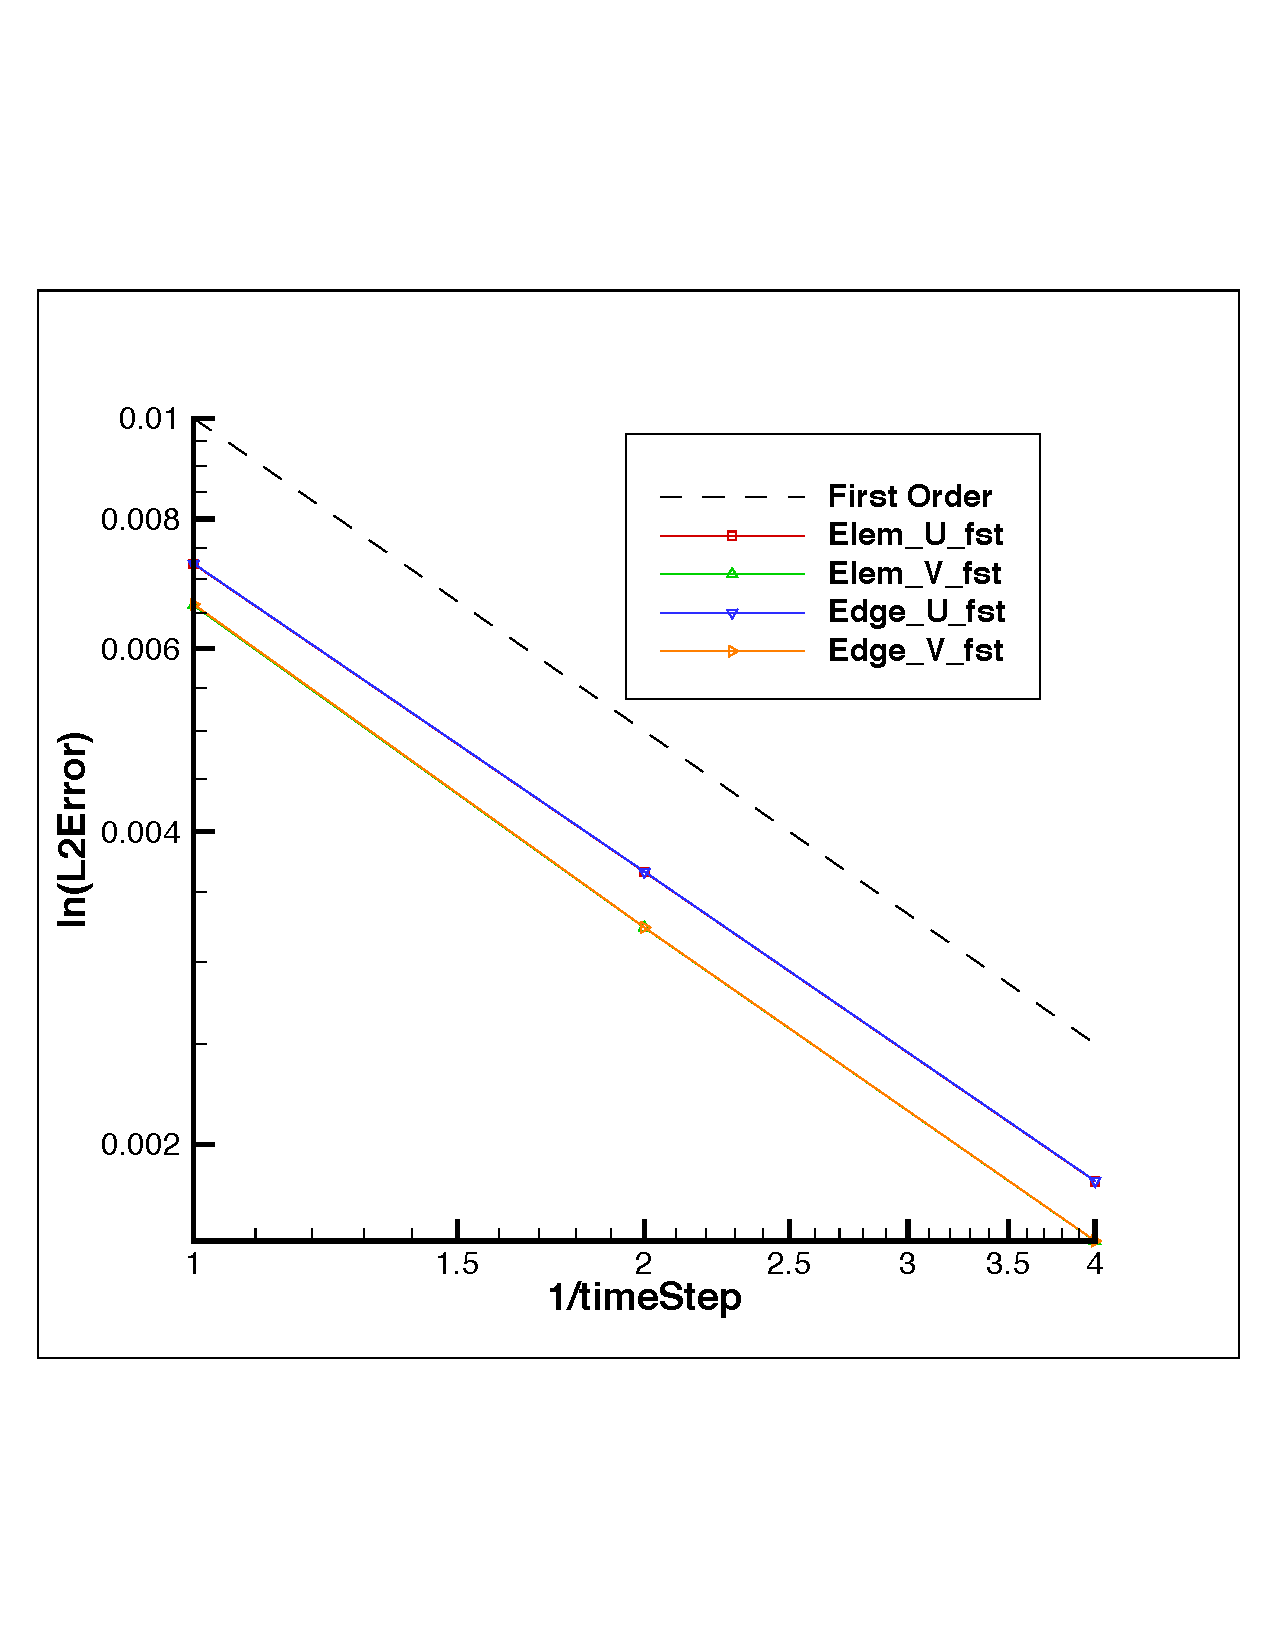
\includegraphics[width=0.6\textwidth]{figures/convTaylorVortexFO.pdf}}
\caption{Error norms as a function of timestep size for the $u$ and $v$
component of velocity using fourth order pressure stabilization with timestep scaling, backward Euler}
\label{fig:fo4thTstep}
\end{figure}

\begin{figure}
\centerline{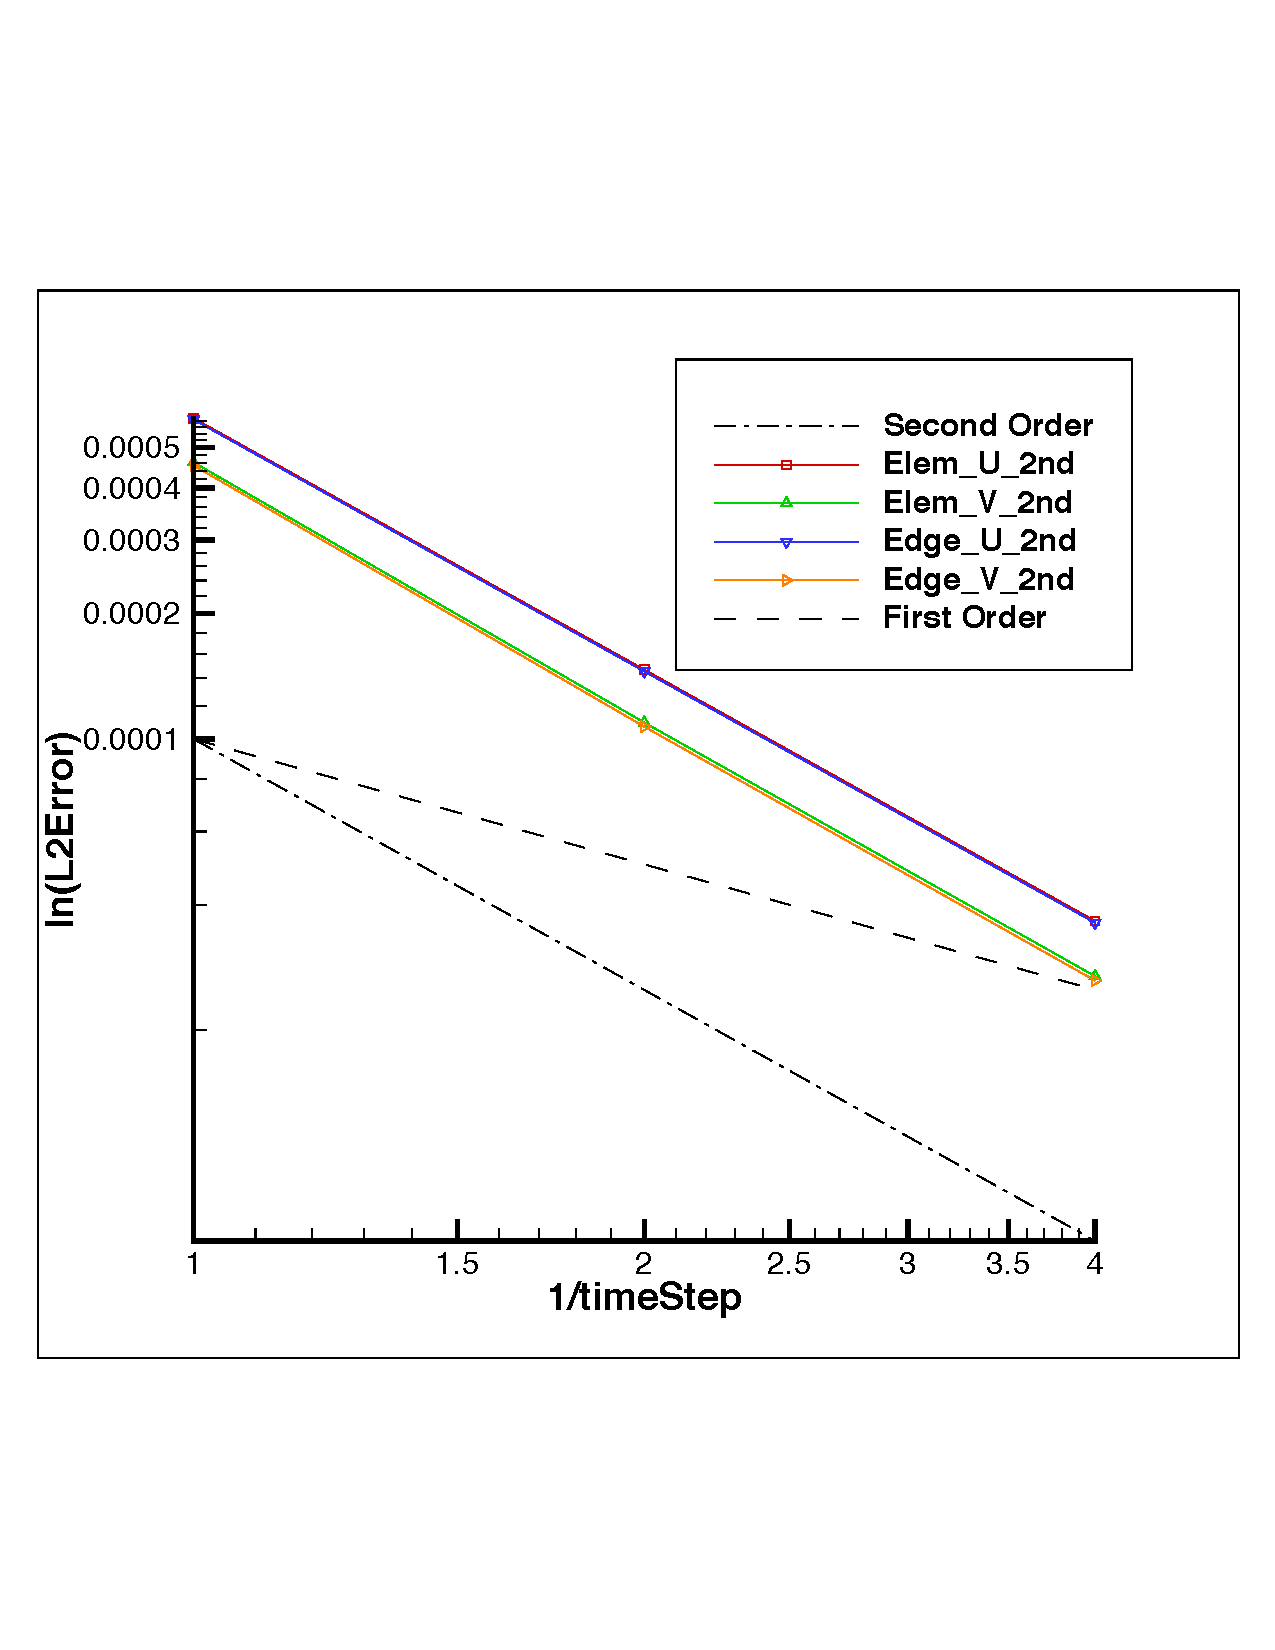
\includegraphics[width=0.6\textwidth]{figures/convTaylorVortexSO.pdf}}
\caption{Error norms as a function of timestep size for the $u$ and $v$
component of velocity using fourth order pressure stabilization with timestep scaling, BDF2}
\label{fig:so4thTstep}
\end{figure}

\begin{figure}
\centerline{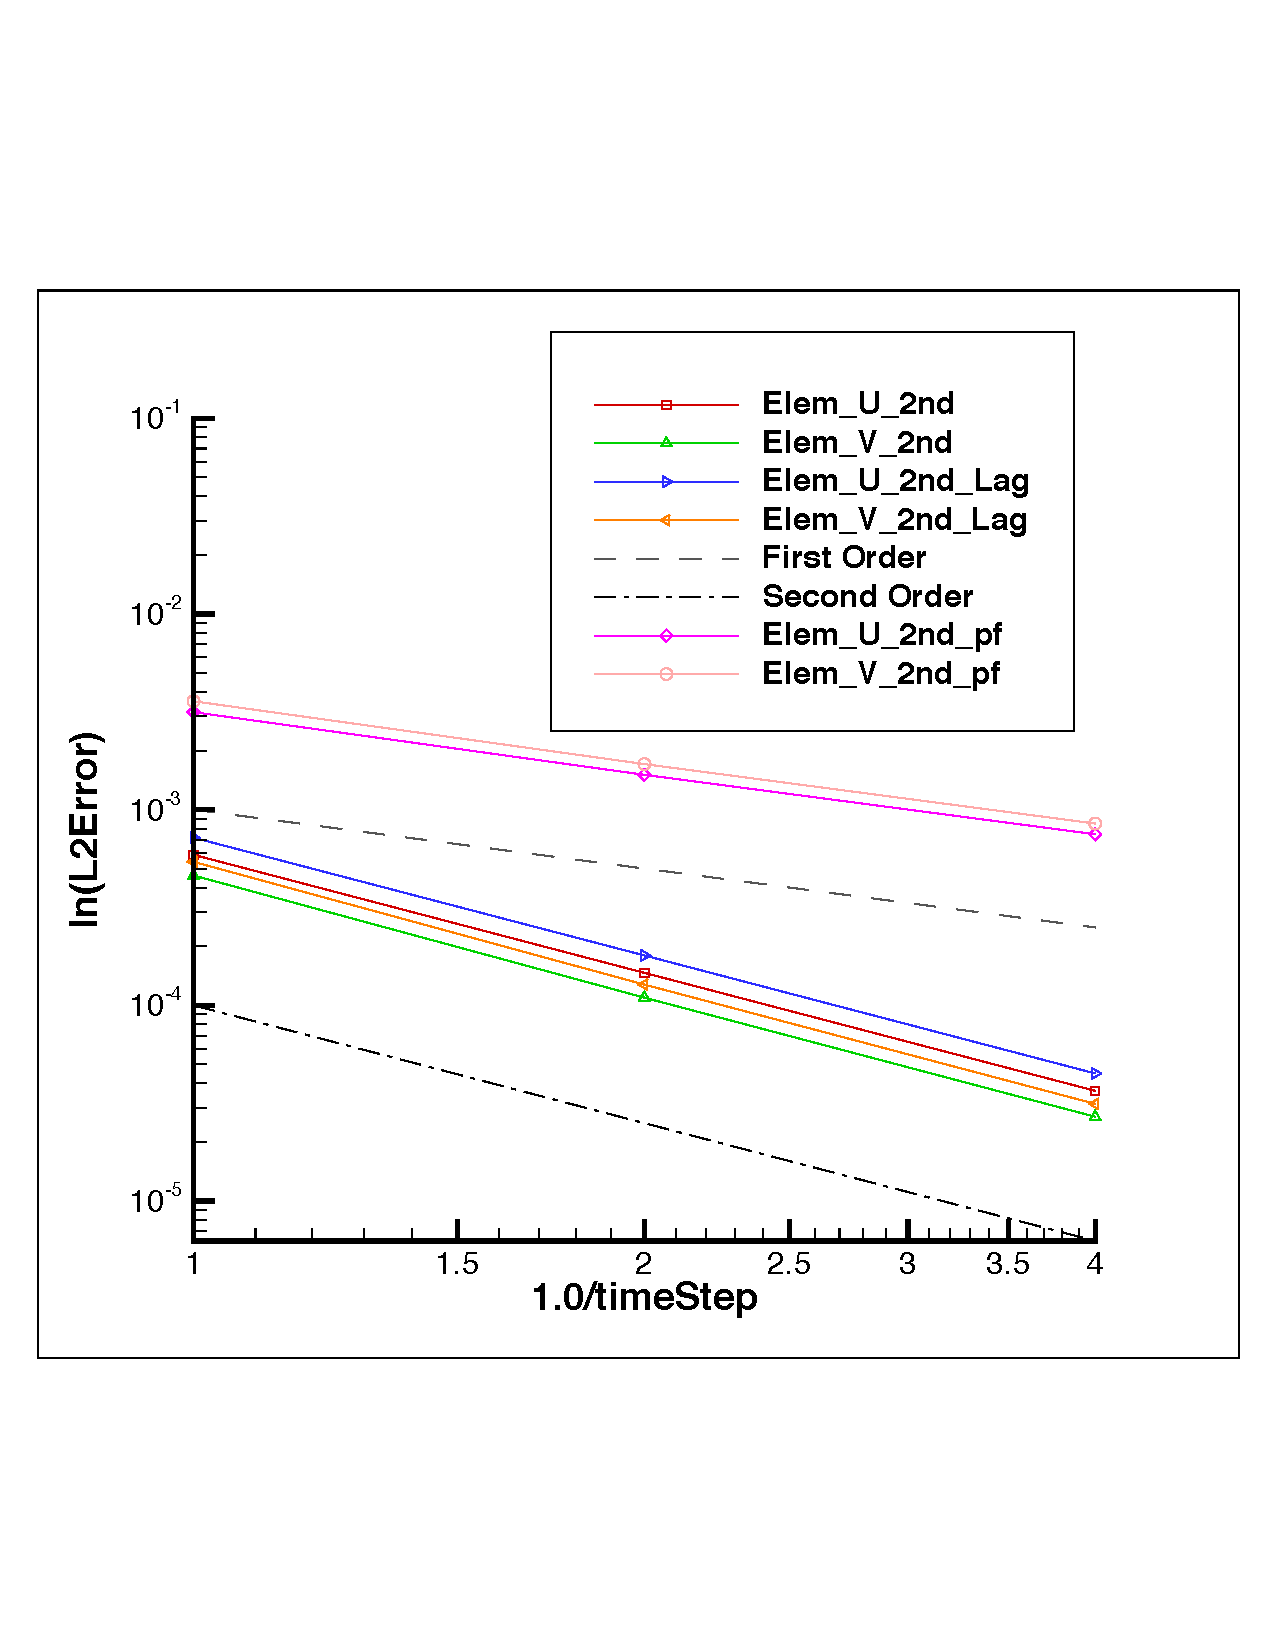
\includegraphics[width=0.6\textwidth]{figures/convTaylorVortexSO_ElemLagElemPf.pdf}}
\caption{Error norms as a function of timestep size for the $u$ and $v$
component of velocity using the lagged projected nodal pressure gradient and pressure-free pressure projection scheme; all with with timestep scaling, BDF2}
\label{fig:hybridTstep}
\end{figure}

\section{Higher Order 2D Steady Uniform Property: Taylor Vortex}

A higher order unstructured CVFEM method has been developed by Domino~\cite{Domino:2014}. 
A 2D structured mesh study demonstrating second order time and third order in space scheme 
has been demosntrated. The work below pushes to unstructured meshes.

\subsection{Projected nodal gradients}
Results show that one must use design order projected nodal gradients. Figure~\ref{fig:pngTempMMS} demonstrates 
a code verification result for a steady thermal manufactured solution comparing lumped and consistent mass
matrix approaches for the projected nodal gradient on a tquad mesh. In the lumped approach, a simple 
explicit algorithm is processed while for the consistent approach, a simple mass matrix inversion equation 
must be solved. The lumped approach is first order while the consistent approach retains second order. Both
Dirichlet and periodic domains display the same order of convergence.

\begin{figure}
\centerline{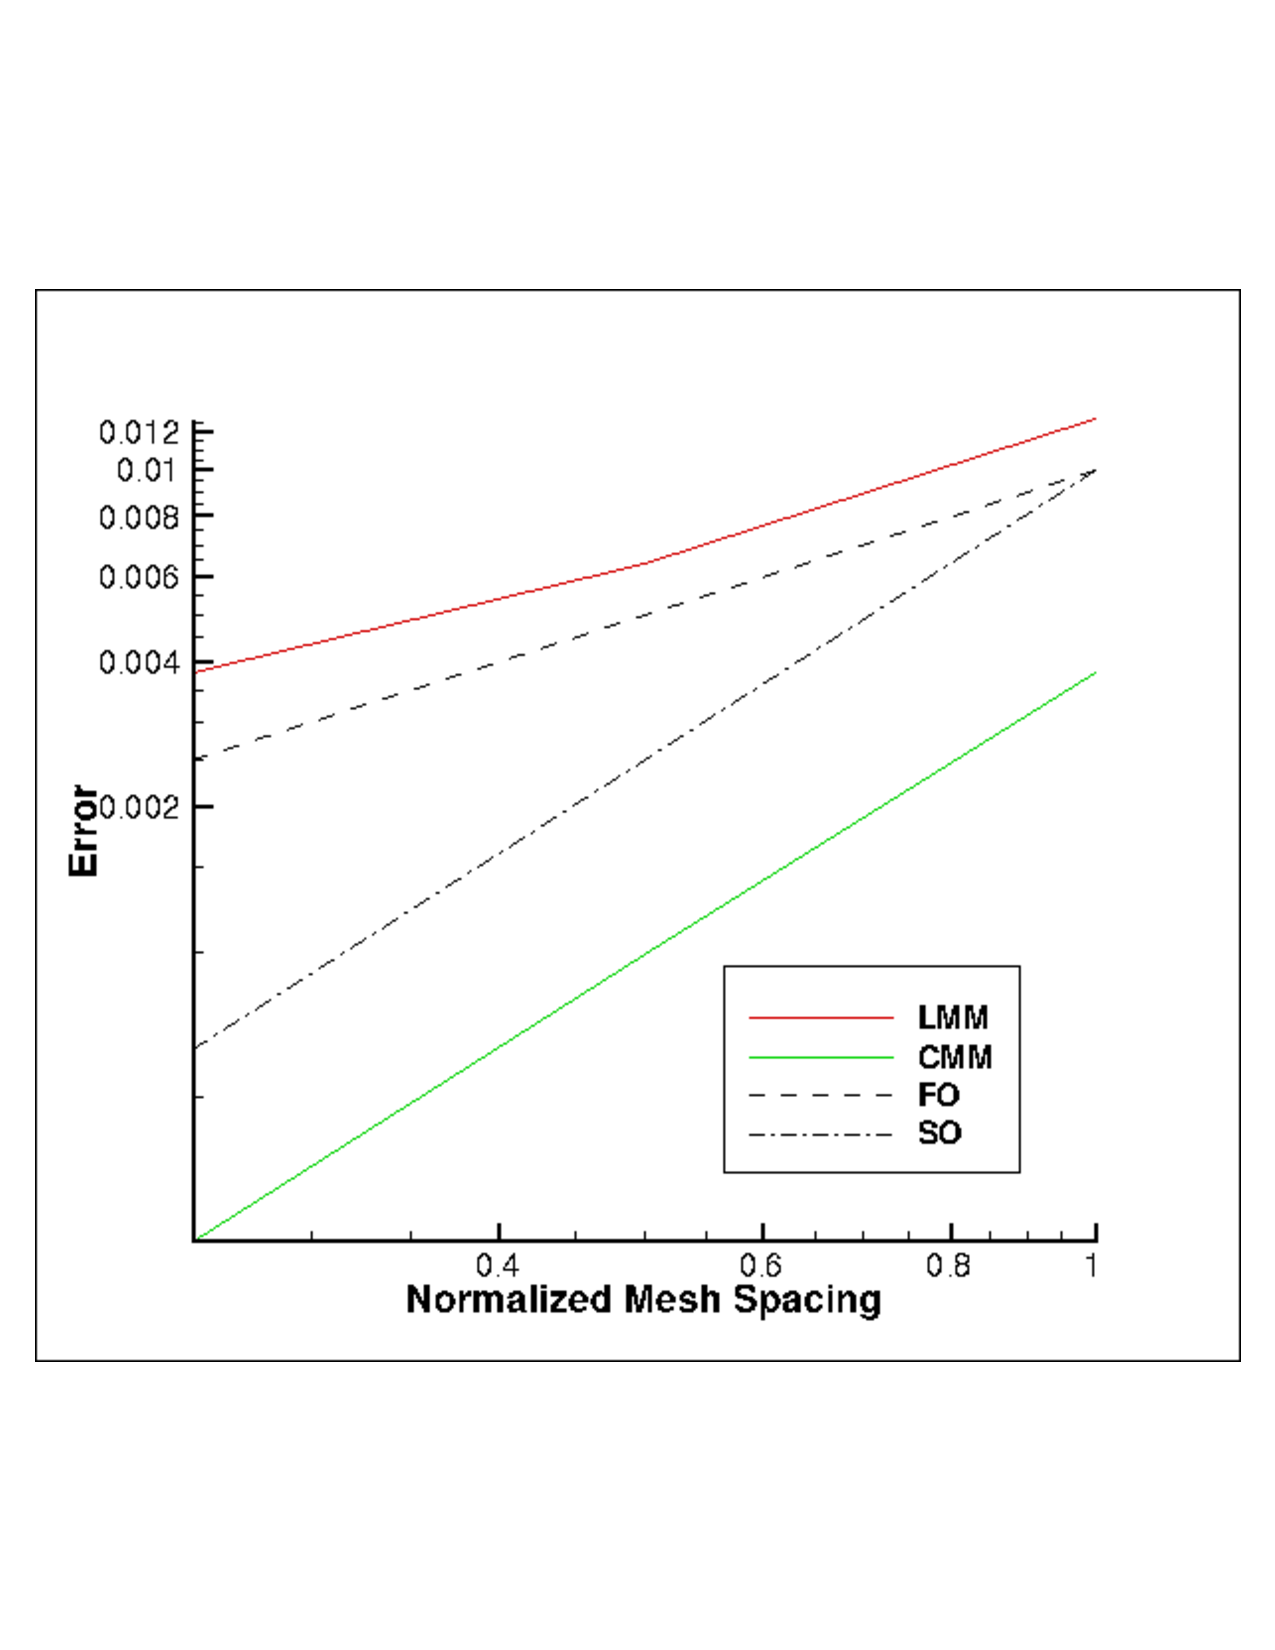
\includegraphics[width=0.6\textwidth]{figures/ho_heatCondMMM_dtdx.pdf}}
\caption{Error norms as a function of mesh size for a CMM and LMM projected nodal gradient.}
\label{fig:pngTempMMS}
\end{figure}

\subsection{Momentum and Pressure}
The same steady taylor vortex was run on a tquad mesh. Figure~\ref{fig:hoSTVMMS} demosntrates the second
order accuracy for the projected nodal graidnet (pressure) and third order for the momentum field. 
Again, dirichlet (inflow) and periodic domains display the same order of convergence.

\begin{figure}
\centerline{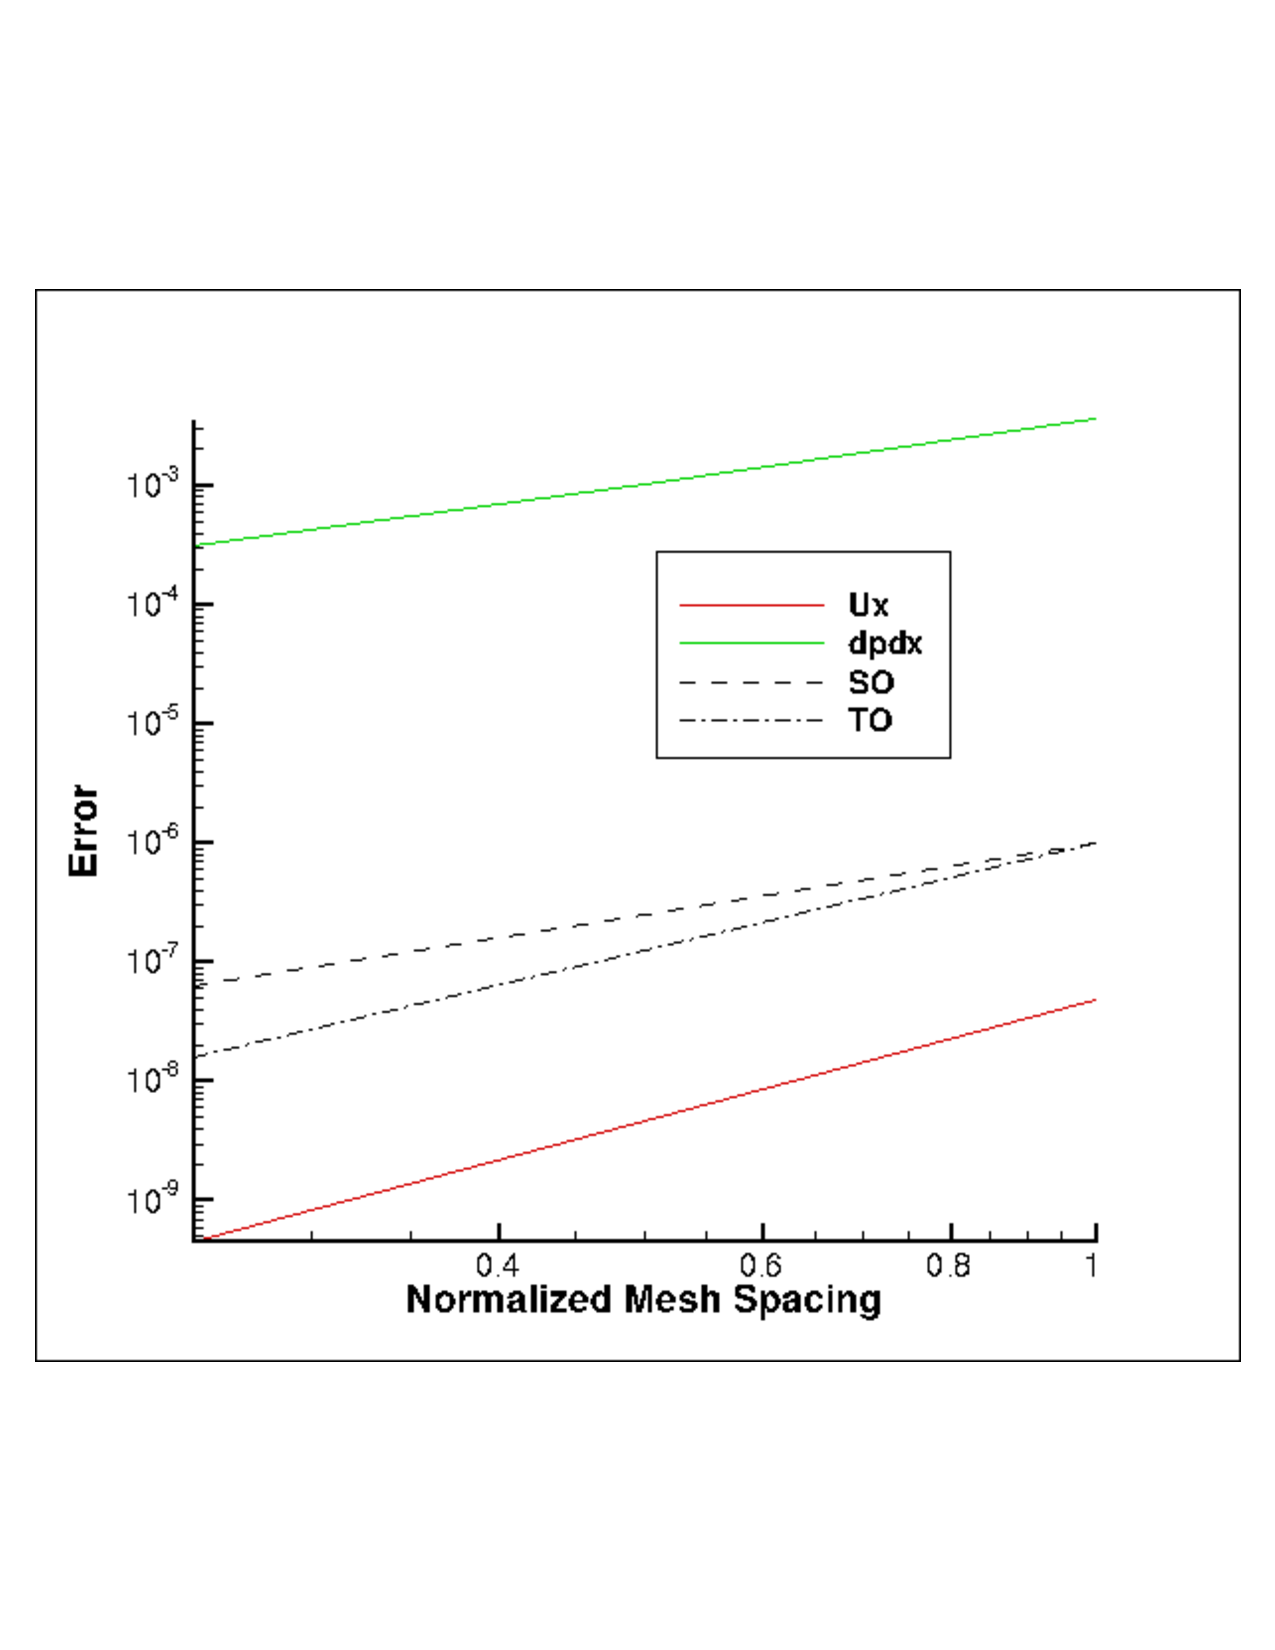
\includegraphics[width=0.6\textwidth]{figures/ho_stvUandDpDx.pdf}}
\caption{Error norms as a function of mesh size for the Steady Taylor Vortex momentum and pressure gradient field.}
\label{fig:hoSTVMMS}
\end{figure}
